% this file is called up by thesis.tex
% content in this file will be fed into the main document

\chapter{Data Exploration} % top level followed by section, subsection
\label{cha:data-exp}

% ----------------------- contents from here ------------------------

The \emph{main} dataset (generated as per the steps outlined in Chapter
\ref{cha:data-prep}) was explored using statistical analysis and
visualizations to observe any patterns and "local trends" that may be
present. The following chapter presents the analysis that were done and the
observations made.

Note that a random sample of only 10\% of the data was taken for the following
visualizations. This is because it is difficult to draw reasonable conclusions
from the plots due to the high number of data points when the entire dataset is
used.

\section{Descriptive Statistics}%
\label{sec:data-exp-desc-stats}

\begin{table}[h]
  \centering
  \caption{Description of columns}
  \label{tab:desc-cols}
  \begin{tabular}{p{1.5cm}p{1.5cm}p{2cm}p{8cm}}
    \hline
    Column & Data type & Unit & Description \\
    \hline
    x, y, z & float & meters (m) & The position within the detector where the hit was detected, they represent the x,y,z coordinates of the hit respectively. \\
    t & float & nano seconds (ns) & The time at which the hit was detected. \\
    label & int & NA & The type of hit, '0' represents noise and '1' represents a neutrino hit \\
    event\_id & int & NA & The id of the event to which the hit is related to. The id itself does not have any meaning, it is simply used to identify hits that originated from the same event. \\
    timeslice & int & NA & The id of the timeslice to which the hit belongs. The id itself does not have any meaning, it is simply used to group hits into discrete bins. \\
    \hline
  \end{tabular}
\end{table}

Table \ref{tab:desc-stats} presents the descriptive statistics of the
\emph{main} dataset. The dataset consists of 7 columns and roughly 4.5 million
rows, Table \ref{tab:desc-cols} provides more information on the columns on the
dataset. The dataset does not contain any \texttt{nan} or \texttt{null} values
except for the \texttt{event\_id} column where rows containing noise hits are
not associated with any event.

\begin{wrapfigure}{r}{0.5\textwidth}
  \centering
  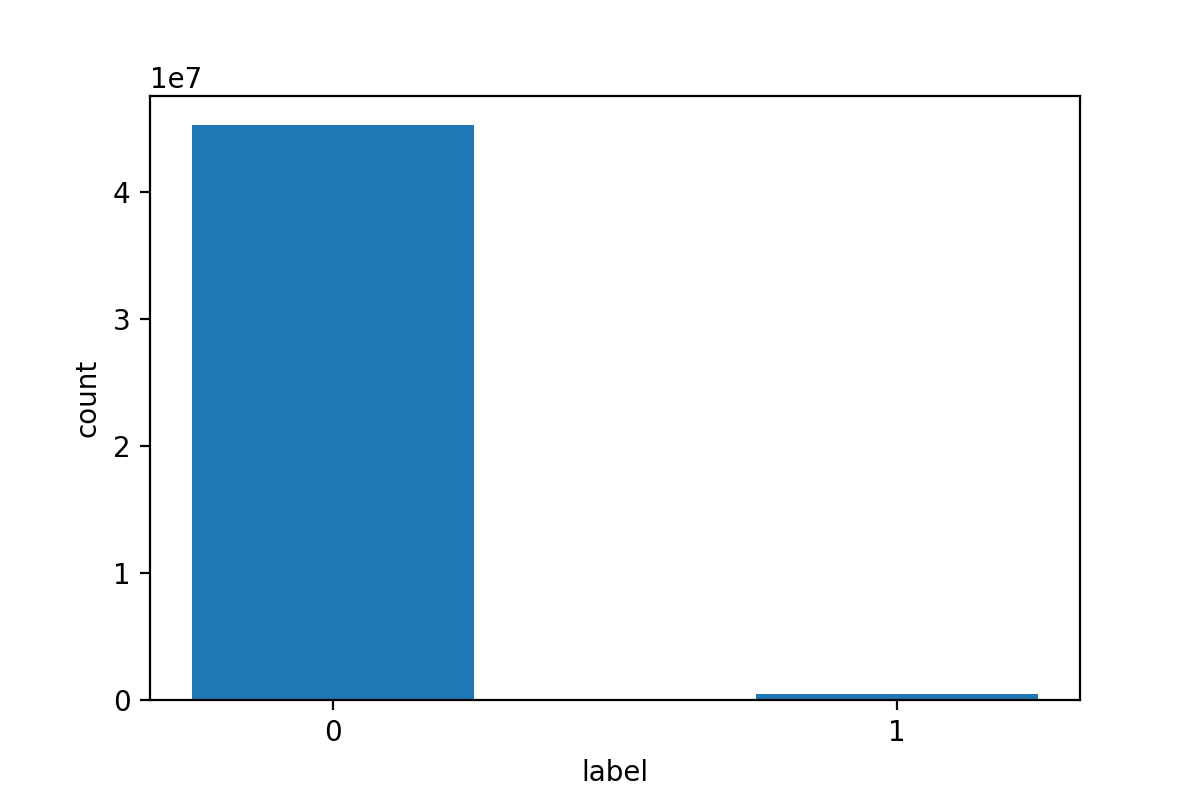
\includegraphics[width=0.9\linewidth]{dist-label.png}
  \caption{Distribution of \texttt{label} column}%
  \label{fig:dist-label}
\end{wrapfigure}

Next, the correlations amongst features is checked, the "Pearson"
correlation is used. Figure \ref{fig:corr} represents the correlation
matrix of all features. No significant correlations are observed
between \texttt{x}, \texttt{y}, \texttt{z} and \texttt{t} which
indicates that ML models may not be able to learn anything from the
dataset without the aid of feature engineering.

\begin{figure}[h]
  \centering
  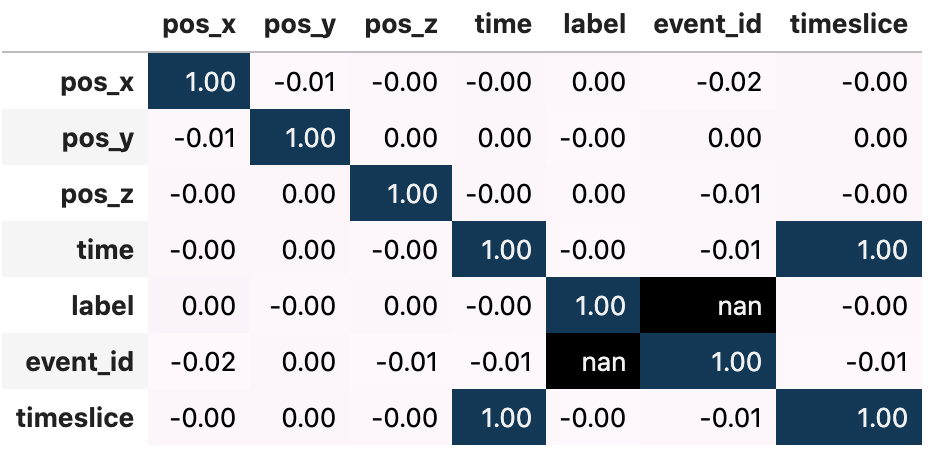
\includegraphics[width=0.8\linewidth]{correlation.png}
  \caption{Correlation matrix of features}
  \label{fig:corr}
\end{figure}

The distribution of the \texttt{label} column is presented in Figure
\ref{fig:dist-label}. A severe class imbalance is noted between events and
noise hits. To be precise, the dataset contains 489906 instances of events
compared to over 4.5 million instances of noise. An effective strategy to
handle the class imbalance will need to be devised during training of models
to prevent the model from overfitting.

\begin{table}[t]
  \centering
  \caption{Descriptive statistics}
  \label{tab:desc-stats}
  \begin{tabular}{lrrrrrrr}
    \hline
          & x & y & z & t & label & event\_id & timeslice \\
    \hline
    count & 4.58e+7 &  4.58e+7 &  4.58e+7 &  4.58e+7 &  4.58e+7 &  489906 &  4.58e+7 \\
    mean  & 1.16e-02 & -1.59e-02 &  1.17e+02 &  5.00e+07 &  1.06e-02 &    2862.00 &  3.33e+03 \\
    std   & 5.12e+01 &  6.22e+01 &  4.86e+01 &  2.89e+07 &  1.02e-01 &    1667.61 &  1.92e+03 \\
    min   & -9.46e+01 & -1.15e+02 &  3.77e+01 &  0.00e+00 &  0.00e+00 &       0.00 &  0.00e+00 \\
    25\%  & -4.50e+01 & -5.79e+01 &  7.40e+01 &  2.50e+07 &  0.00e+00 &    1392.25 &  1.66e+03 \\
    50\%  & 1.30e+00 & -4.18e+00 &  1.21e+02 &  5.00e+07 &  0.00e+00 &    2887.00 &  3.33000e+03 \\
    75\%  & 4.04e+01 &  4.85e+01 &  1.60e+02 &  7.50e+07 &  0.00e+00 &    4304.75 &  5.00000e+03 \\
    max  & 9.62e+01 &  1.05e+02 &  1.96e+02 &  1.01e+08 &  1.00e+00 &    5734.00 &  6.77e+03 \\
    \hline
  \end{tabular}
\end{table}

\section{Verification of Bias}%
\label{sec:data-exp-verification-bias}

The \emph{events} dataset is synthetically generated using simulations. As such,
it is likely that the event hits in each timeslice may occur at a specific
time such as at the beginning, middle or end of the timeslice. Having such
a pattern in the dataset may bias the model since it may learn this pattern and
thus fail to generalize. If this pattern does exist in the dataset, corrective
measures need to be taken such that the event hits in each timeslice are
uniformly distributed.

To verify the existence of such patterns in the dataset, the mean time
of event hits across all events was visualized as a scatter plot as
depicted by Figure \ref{fig:bias-verification}. A uniform distribution
is noted with no visible patterns. Thus no bias exists in the dataset
and it is deemed suitable for further analysis.

\begin{wrapfigure}{l}{0.5\textwidth}
  \centering
  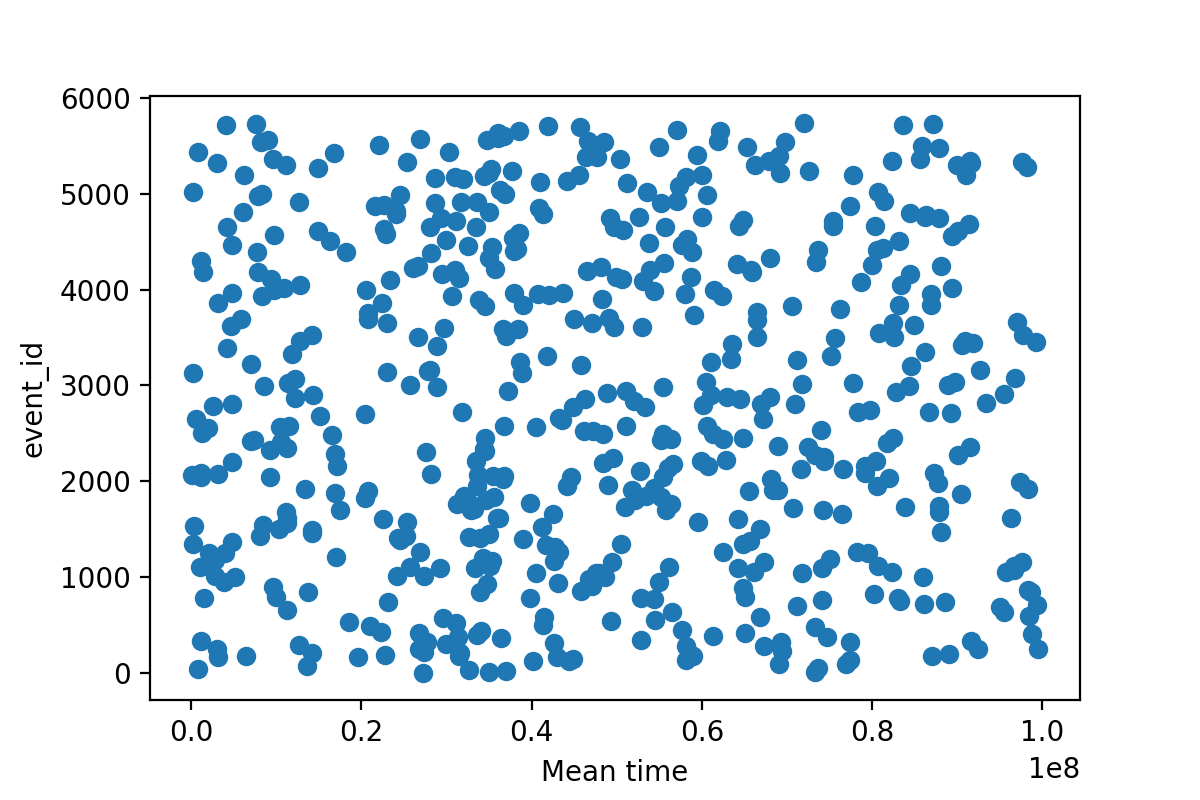
\includegraphics[width=0.9\linewidth]{bias-verification.png}
  \caption{Verification of Bias}%
  \label{fig:bias-verification}
\end{wrapfigure}

\section{Exploration of Interesting Timeslices}%
\label{sec:data-exp-interesting-timeslices}

Figure \ref{fig:dist-hits-per-timeslice} represents to total number of
event hits per timeslice. The dataset is discretized into 6759
timeslices of which 2783 timeslices contain only noise hits. This is
corroborated by Figure \ref{fig:dist-hits-per-timeslice} which
presents a skewed distribution where many timeslices contain few to no
event hits and few timeslices contain a high number of event hits.

\begin{wrapfigure}{r}{0.5\textwidth}
  \centering
  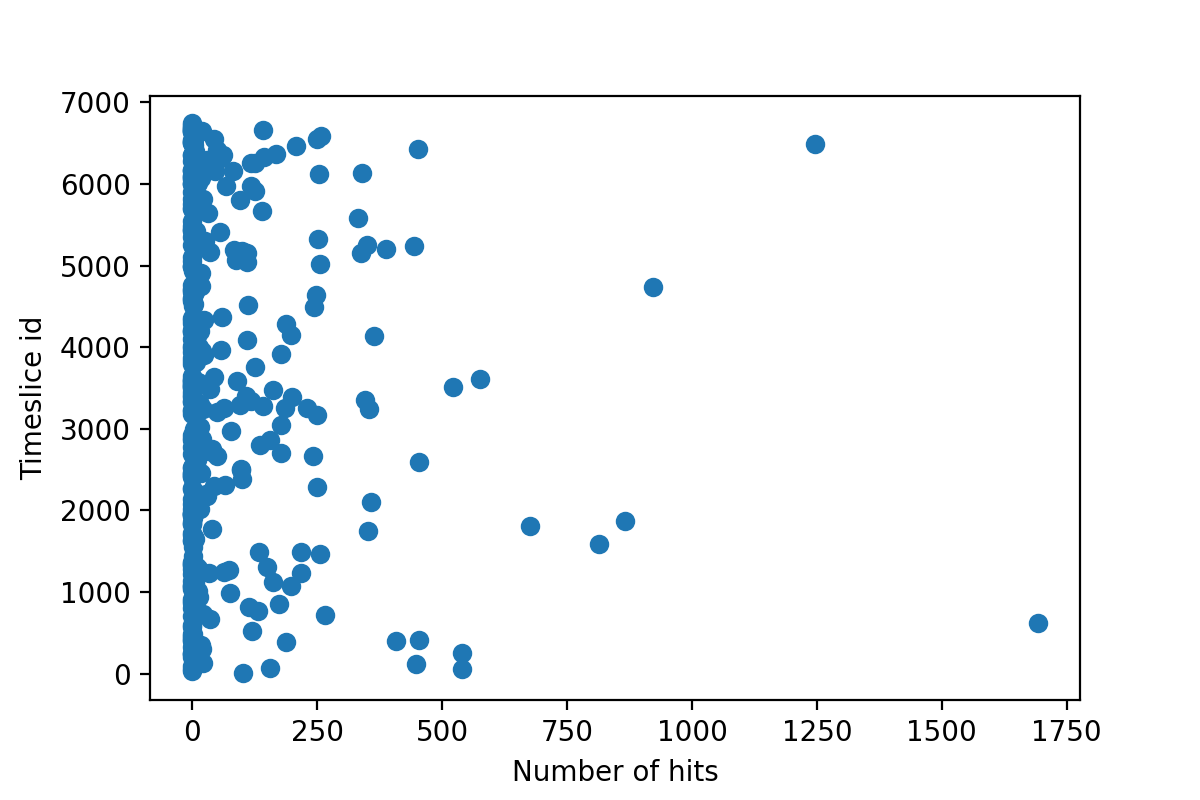
\includegraphics[width=0.9\linewidth]{dist-hits-per-timeslice.png}
  \caption{Distribution of event hits per timeslice}%
  \label{fig:dist-hits-per-timeslice}
\end{wrapfigure}

Figure \ref{fig:dist-timeslice-largest} depicts a scatter plot of
\emph{timeslice 615} which contains the largest number of event hits.
It is observed that event hits occur close to each other in space and
time (represented by the yellow, blue and green points) whilst
background hits are uniformly distributed in space and time
(represented by the purple points).

\begin{figure}[h]
  \centering
  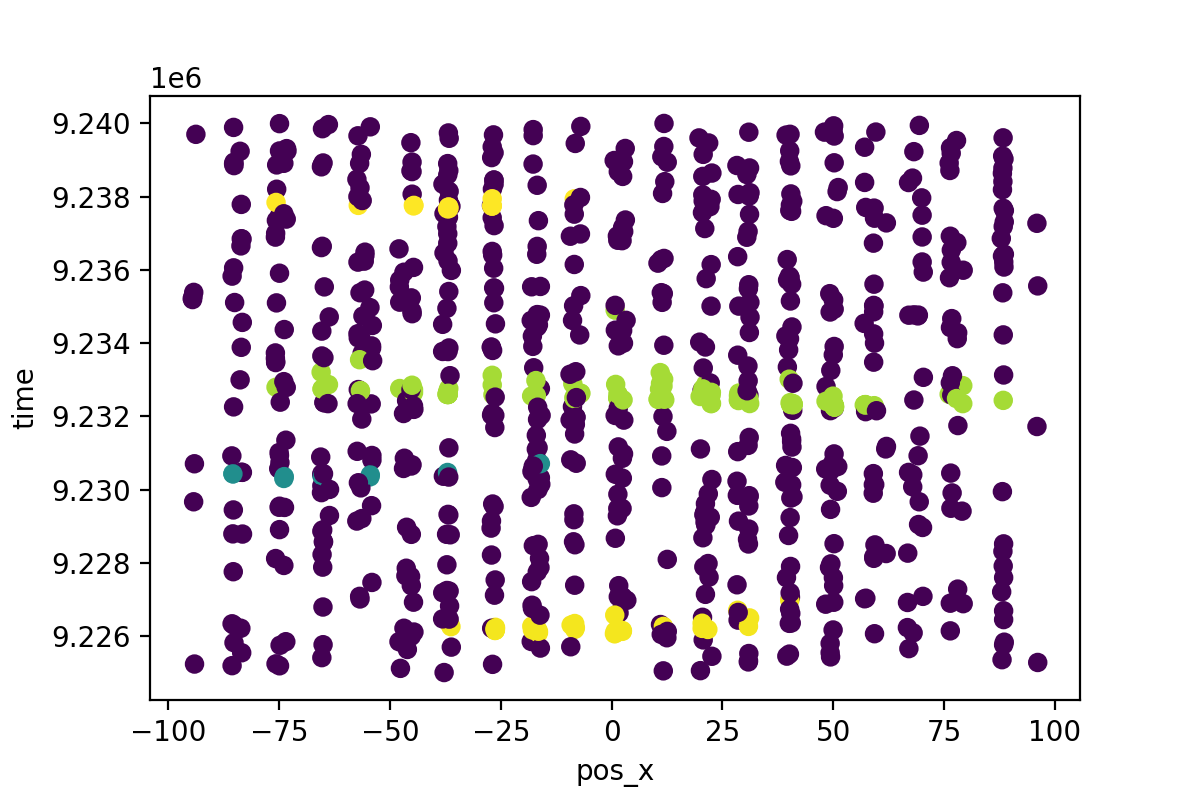
\includegraphics[width=0.9\linewidth]{dist-timeslice-largest-posx-time-eventid.png}
  \caption{Distribution of Timeslice 615}%
  \label{fig:dist-timeslice-largest}
\end{figure}


% ---------------------------------------------------------------------------
% ----------------------- end of thesis sub-document ------------------------
% ---------------------------------------------------------------------------
